\documentclass[tikz,border=5pt]{standalone}
\usepackage{tikz}
\usetikzlibrary{arrows.meta,positioning}
\definecolor{nebula}{HTML}{6366F1}
\definecolor{spark}{HTML}{14B8A6}
\definecolor{ink}{HTML}{334155}
\begin{document}
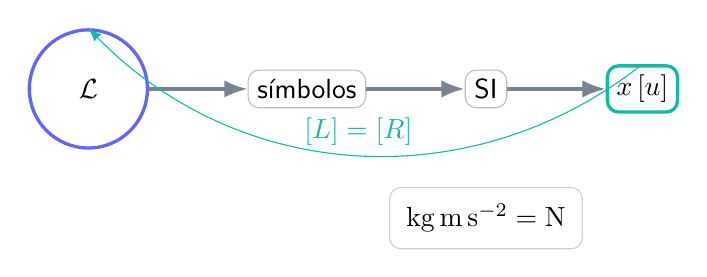
\begin{tikzpicture}[font=\sffamily,>=Latex,node distance=1.25cm]
  \node[draw=nebula,very thick,circle,minimum size=1.5cm] (law) {$\mathcal L$};
  \node[draw=ink!35,rounded corners=4pt,right=of law] (sym) {símbolos};
  \node[draw=ink!35,rounded corners=4pt,right=of sym] (si) {SI};
  \node[draw=spark,very thick,rounded corners=4pt,right=of si] (res) {$x\,[u]$};
  \draw[->,very thick,ink!65] (law)--(sym); \draw[->,very thick,ink!65] (sym)--(si);
  \draw[->,very thick,ink!65] (si)--(res);
  \draw[->,spark,bend left=42] (res.north) to node[above] {$[L]=[R]$} (law.north);
  \node[below=1cm of si,draw=ink!25,rounded corners=4pt,fill=white,inner sep=6pt]
    {$\mathrm{kg\,m\,s^{-2}}=\mathrm N$};
\end{tikzpicture}
\end{document}
